% ─── Slide: Analog MVM Signal Path ───────────────────────────────────────────
\begin{frame}{Math model of an optical linear layer}

  \vfill
  \begin{center}
  \resizebox{0.8\linewidth}{!}{%
  \begin{tikzpicture}[
      every node/.style={font=\small},
      q/.style={draw=mybluedark, rounded corners=3pt, fill=myblue!22,
                minimum width=1.9cm, minimum height=0.72cm, align=center},
      tile/.style={draw, rounded corners=3pt, fill=mybluedark!15, text=mybluedark,
                   minimum width=2.2cm, minimum height=1.0cm, align=center},
      adc/.style={draw=myorange, line width=1.5pt, rounded corners=3pt,
                  fill=myorange!25, minimum width=1.7cm, minimum height=0.72cm,
                  align=center},
      arr/.style={-{Latex[length=2.5mm]}, thick, mybluedark}
    ]
    % Reserve a constant bounding box so overlays don't shift the diagram
    \useasboundingbox (-0.5, -3.4) rectangle (11.5, 3.4);

    \node (w)  at (0,   1.1) {$w$};
    \node[q] (qw) at (2.1,  1.1) {Digital\\quantiser};
    \node (wb) at (4.0,  1.1) {$\hat w$};

    \node (x)  at (0,  -1.1) {$x$};
    \node[q] (qx) at (2.1, -1.1) {Digital\\quantiser};
    \node (xb) at (4.0, -1.1) {$\hat x$};

    \draw[arr] (w)--(qw);   \draw[arr] (qw)--(wb);
    \draw[arr] (x)--(qx);   \draw[arr] (qx)--(xb);

    \node[tile] (T) at (6.2, 0) {Optical MVM\\$y{=}\langle\hat w,\hat x\rangle$};
    \draw[arr] (wb) -- (T.north west);
    \draw[arr] (xb) -- (T.south west);

    \node (y)  at (8.05, 0) {$y$};
    \draw[arr] (T)--(y);

    \node[adc] (A) at (9.4, 0) {ADC\\$\lfloor y/\delta\rfloor$};
    \draw[arr] (y)--(A);

    \node (yb) at (11.0, 0) {$\hat y$};
    \draw[arr] (A)--(yb);

    % ── Overlay parts (interactive build-up) ────────────────────────────
    \only<2>{
      \node[anchor=south] at (4.0,  1.6)
        {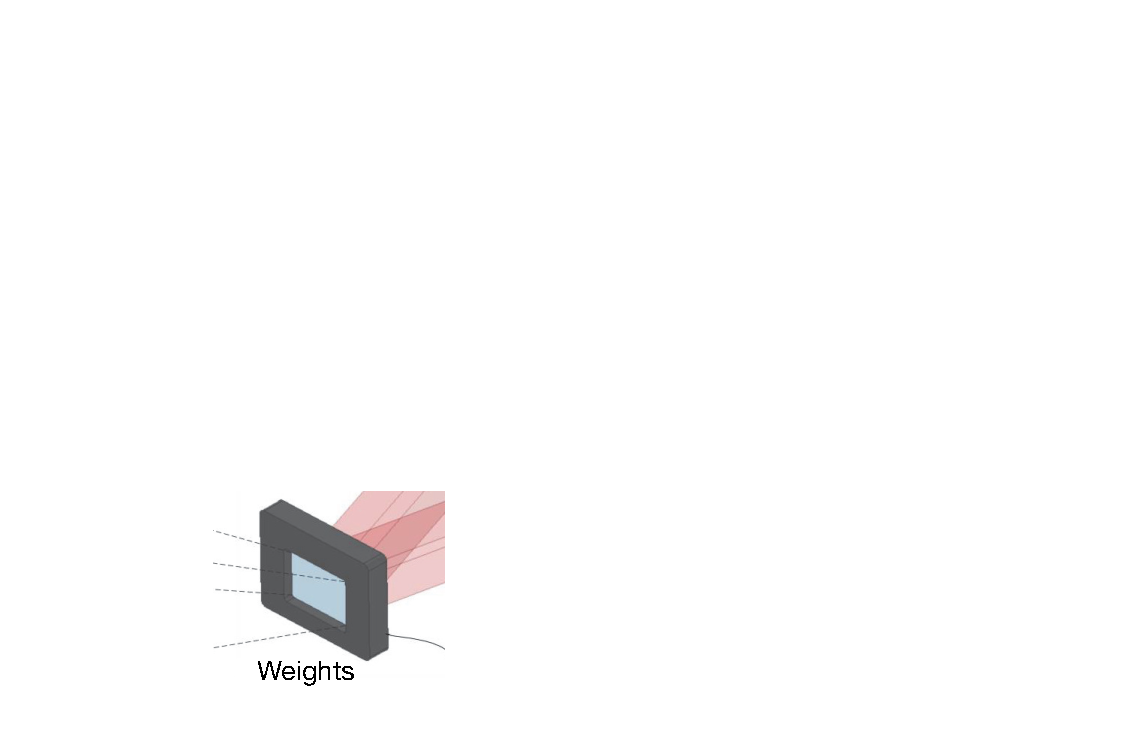
\includegraphics[width=2cm]{figs/parts/weights.pdf}};
      \node[anchor=north] at (4.0, -1.6)
        {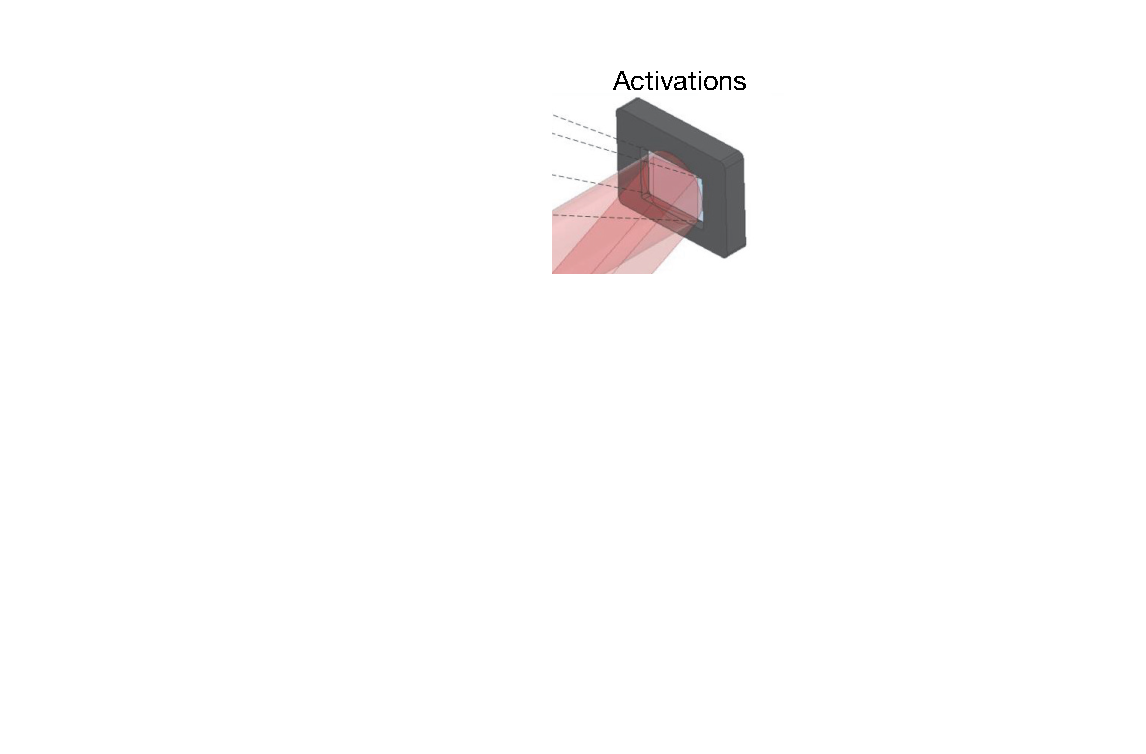
\includegraphics[width=2cm]{figs/parts/activations.pdf}};
    }
    \only<3>{
      \node[anchor=south] at (6.2, 0.7)
        {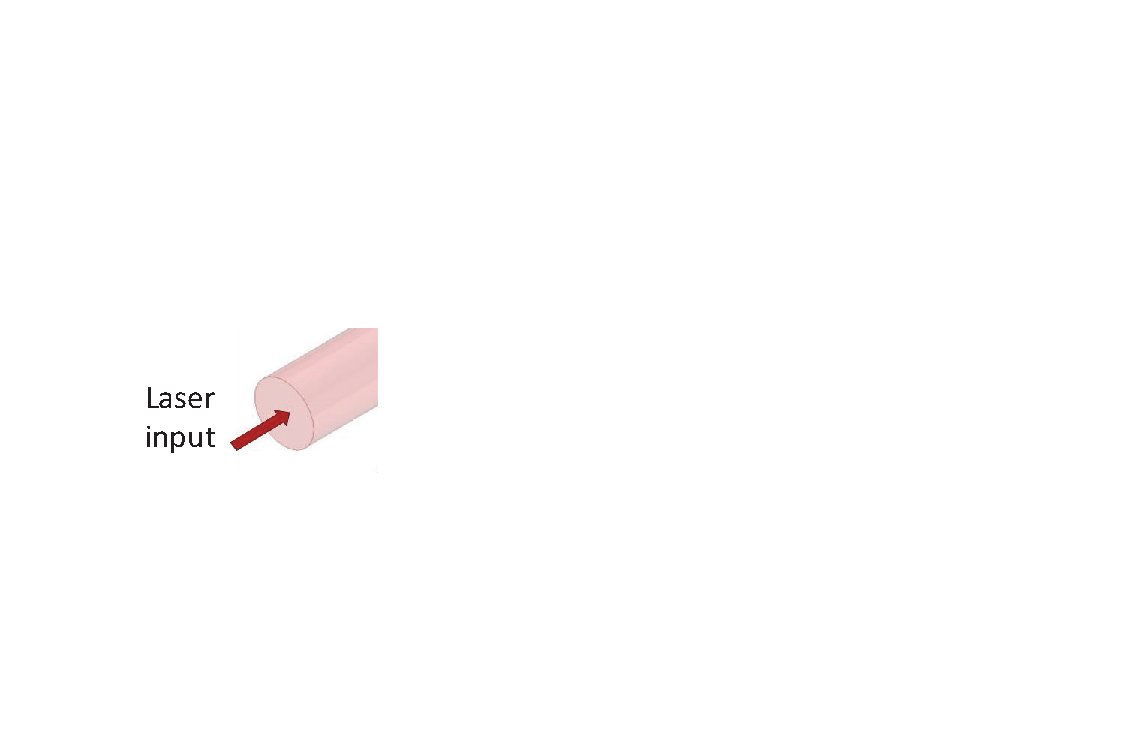
\includegraphics[width=2.4cm]{figs/parts/mvm.pdf}};
    }
    \only<4>{
      \node[anchor=south] at (9.4, 0.55)
        {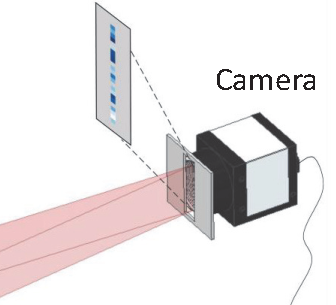
\includegraphics[width=2cm]{figs/parts/adc.pdf}};
    }

  \end{tikzpicture}}
  \end{center}
  \vfill

  \begin{tikzpicture}[remember picture, overlay]
    \node[anchor=south west, inner sep=0pt]
      at ([xshift=0.6cm, yshift=0.5cm]current page.south west) {%
      {\scriptsize\color{mygray}\itshape
        \begin{tabular}{@{}l@{}}
          $^{*}$MVM — matrix-vector multiplication. \\
          $^{*}$ADC — analog-to-digital converter.
        \end{tabular}}};
    \node[anchor=south east, inner sep=0pt]
      at ([xshift=-0.5cm, yshift=0.5cm]current page.south east) {%
        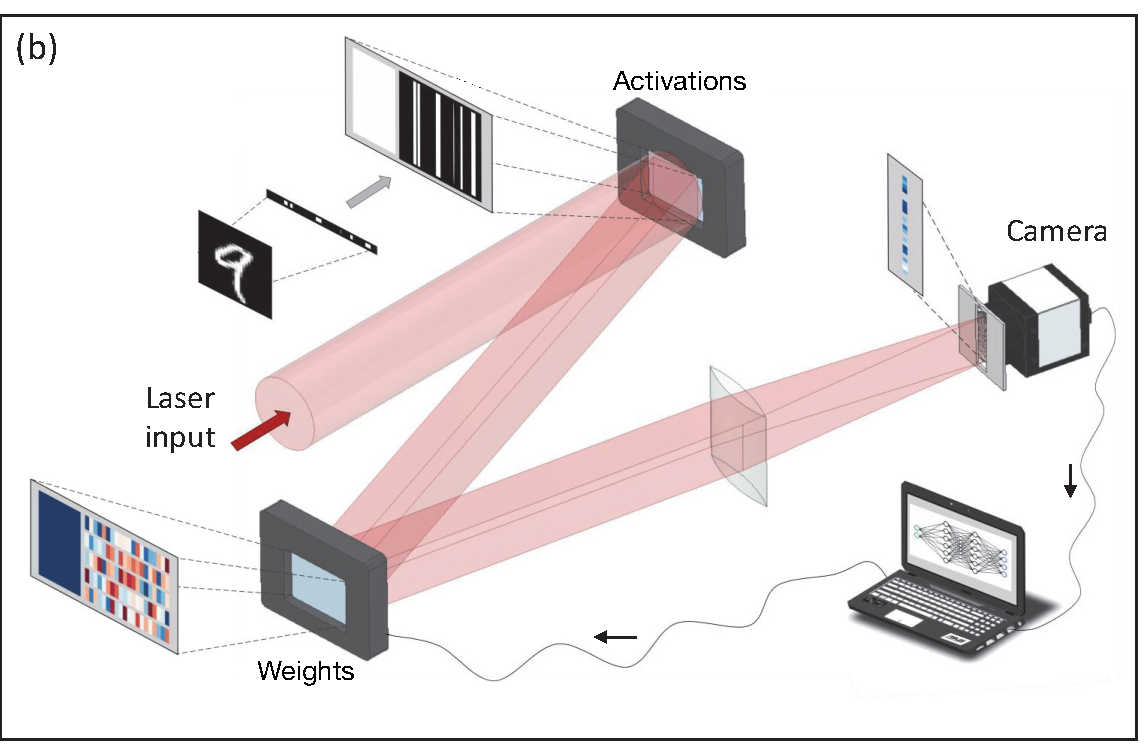
\includegraphics[width=4.2cm,keepaspectratio]{figs/Fig1b.pdf}};
  \end{tikzpicture}

  \note{Показываю общую схему. Линейный слой проходит через два ключевых этапа: сначала квантизация весов и активаций, потом аналоговое умножение матриц, результат которого читается через АЦП.}

\end{frame}
